\documentclass{beamer}
\usepackage[utf8]{inputenc}
% \usepackage{polski}
% \usepackage[polish]{babel}
\usepackage[T1]{fontenc}
\usepackage{tikz}
\usepackage{tikzducks}
% \usetikzlibrary{decorations.pathmorphing}
\usepackage{multimedia}
\usepackage{graphicx}
\usepackage[justification=centering]{caption}
\usepackage{textcomp}
\usepackage{appendixnumberbeamer}
\usepackage{qrcode}
% \usepackage[natbib, language=polish, sorting=none]{biblatex}
% \addbibresource{lio.bib}
\usepackage{hyperref}
%\usepackage[width=\textwidth]{animate}
%\usepackage{chemformula}
\usepackage{sidecap}
\usepackage{multirow}
%\usepackage{rotating}
%\usepackage{anyfontsize} % change font size for semposiwko
\usepackage{siunitx}
\usepackage{soul}



\usepackage[natbib, language=polish, sorting=none]{biblatex}
\addbibresource{lio.bib}
\renewcommand*{\bibfont}{\scriptsize}

\usetheme{Szeged}
\usecolortheme{whale}
\setbeamercolor{palette primary}{bg=violet!80!black,fg=white}
\setbeamercolor{palette secondary}{bg=violet!60!black,fg=white}
\setbeamercolor{palette tertiary}{bg=violet!40!black,fg=white}
\setbeamercolor{palette quaternary}{bg=violet!20!black,fg=white}
\setbeamercolor{structure}{fg=violet!60!black}
\setbeamertemplate{caption}{\insertcaption}
\makeatletter
\beamer@theme@subsectionfalse
\makeatother
% \setbeamertemplate{headline}{
%   \begin{beamercolorbox}[wd=.9\paperwidth]{headline}
%     \vspace{1.5ex}
%     \insertsectionnavigationhorizontal
%     \vspace{1.5ex}
%   \end{beamercolorbox}
% }

\linespread{0.6}

\setbeamertemplate{background}%
{%
    \begin{tikzpicture}[remember picture,overlay]{\node[yshift=1.5cm,xshift=-2cm,opacity=0.1] at (current page.south east)
      {
      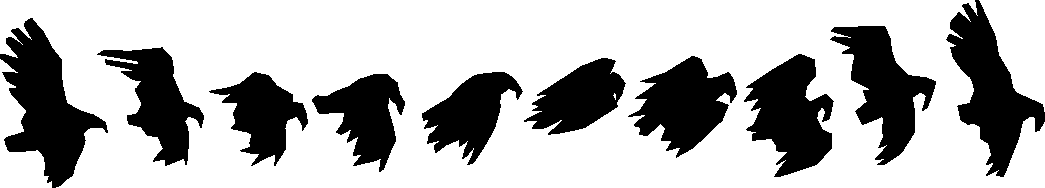
\includegraphics[scale=0.4, angle=20]{ptaki.pdf}
      }
      ;
    \node[yshift=1.0cm,xshift=0.6cm] (logopos) at (current page.south west) {{\begin{tikzpicture}\shuffleducks\duck[signpost=\insertframenumber, \randomhead,scale=.4]\end{tikzpicture}}};
    \pgfmathsetmacro{\progress}{360*(\insertframenumber)/(\inserttotalframenumber)};
    \draw[line width=0.2*3pt] ([xshift=0.55cm] logopos)  arc[radius=0.55cm, start angle=0, end angle=\progress];
    \fill ([shift={(\progress:0.55cm)}] logopos) circle(1pt);

    }
        \end{tikzpicture}
    
}

\newcommand{\SeMPowisko}{%
\large S\normalsize%
\kern-.3em \lower.2ex\hbox{e}%
\lower.2ex\hbox{\large M\normalsize}%
\kern-.1em \raise.1ex\hbox{\large P\normalsize}%
\kern-.3em \lower.2ex\hbox{o}%
\kern-.2em \raise.2ex\hbox{w}%
\lower.2ex\hbox{i}%
s%
\raise.2ex\hbox{k}%
\kern-.3em \lower.2ex\hbox{o}%
}

\setbeamerfont{caption}{size=\tiny}

\title[Papier w zastosowaniach elektronicznych i~optoelektronicznych$^1$]{Papier w zastosowaniach elektronicznych i~optoelektronicznych\footnote{sygnały optyczne $\leftrightarrow$ sygnały elektroniczne}}
% \subtitle{Przegląd niektórych eksperymentów}
\author[M. Winiarski]{Mateusz Winiarski}
\institute[fizyk UJ]{fizyka IV-I, WFAIS}
\date[dzisiaj]{13 maja 2024\\dzisiaj}

\begin{document}

\frame{\titlepage}

\section{Papier}
        \begin{frame}{Wady \hfill i \hfill zalety}
\begin{columns}

\begin{column}{0.5\textwidth}
    \begin{itemize}
        \item \only<1>{nie przewodzi prądu} \only<2>{\st{nie~przewodzi~pradu}}
        \item jest nieprzezroczysty
        \item jest chropowaty
        \item jest porowaty i~niewodoodporny
    \end{itemize}
\end{column}\pause
\begin{column}{0.5\textwidth}
    \begin{itemize}
        \item jest tani (tańszy nawet niż plastik)
        \item jest łatwy w produkcji
        \item jest ekologiczny
        \item jest giętki
        \item nie przewodzi prądu
    \end{itemize}
    % \pause
    \end{column}
% \begin{column}{0.5\textwidth}
%     \begin{figure}
%         \centering
%         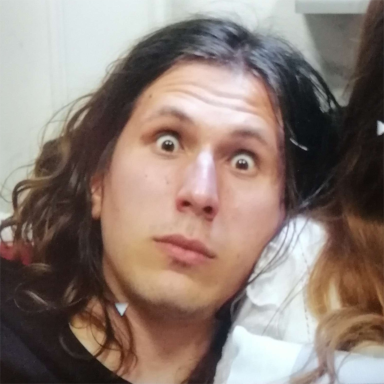
\includegraphics[width=0.9\linewidth]{firlejpatrzy.png}
%         \caption{Your reaction to that information}
%     \end{figure}
% \end{column}
\end{columns}
\end{frame}

\begin{frame}{Jak pozbyć się wad}
        \begin{figure}[h]
        \centering
        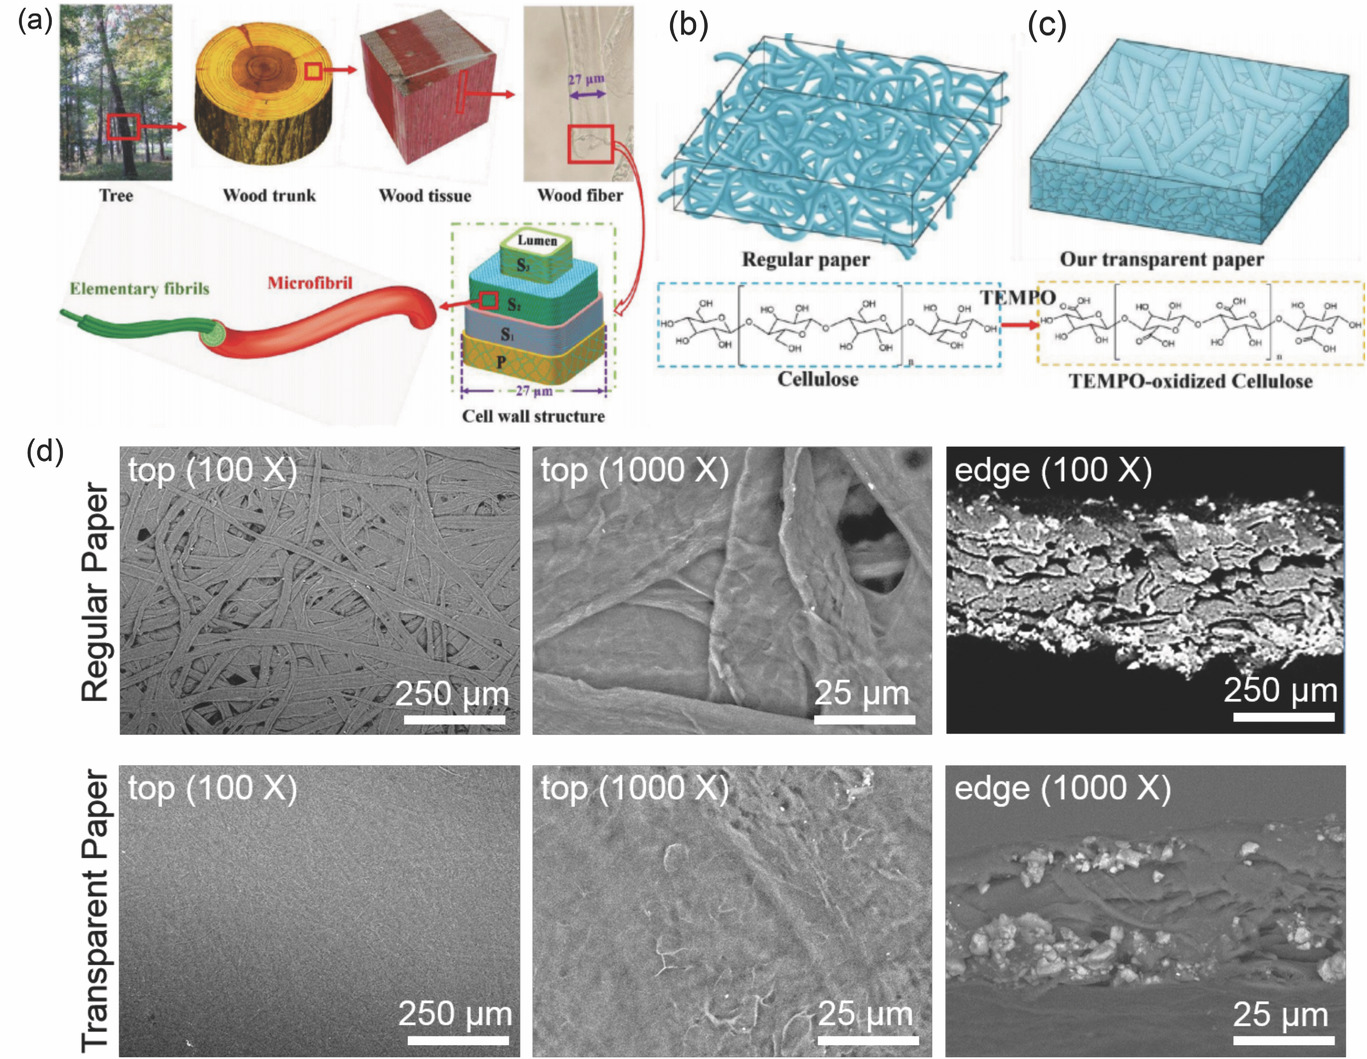
\includegraphics[width=0.7\linewidth]{fig1}
        \caption{a) Schematic showing the hierarchical structure of a tree. b,c) Schematic illustrating structure of (b) a regular paper and (c) TEMPO-oxidized wood fibers and the corresponding chemical structures of the constituent cellulose. d) SEM images of a regular paper and TEMPO-oxidized transparent paper. The transparent paper shows fewer porous air cavities and thus higher packing density of cellulose fibers than the regular paper, resulting in high transmission.\\
        \typeout{}
        [source: \url{https://doi.org/10.1002/adma.200803174}]
        }
        % \label{fig:enter-label}
        
    \end{figure}
\end{frame}

\begin{frame}{Lista zastosowań}
\begin{tabular}{@{$\blacktriangleright$ }l @{$\quad\to\quad$ } l}
    fotowoltaika & pokrycia antyodblaskowe \\
    obwody elektroniczne & FETy, elektrolity \\
    ekrany & podłoża OLEDów i ekranów dotykowych \\
    magazynowanie energii & elektrody, separatory \\
    anteny & podłoża \\
\end{tabular}
\end{frame}


\section{Fotowoltaika}

\begin{frame}{Fotowoltaika}
    \begin{itemize}
        \item problem: utrata światła związana z odbiciem
        \item rozwiązanie: warstwy antyodblaskowe
    \end{itemize}
    \begin{columns}
        \begin{column}{0.5\textwidth}
            \begin{itemize}
            \item materiały:
            \begin{itemize}
                \item błony dielektryczne
                \item nanostruktury krzemowe
                \item materiały plazmoniczne
            \end{itemize}
            \end{itemize}
        \end{column}
        \begin{column}{0.5\textwidth}
            \begin{itemize}
            \item wady:
            \begin{itemize}
                \item wysoka cena
                \item właściwości silnie zależne od kąta padania lub długości fali
            \end{itemize}
            \end{itemize}
        \end{column}
    \end{columns}
\end{frame}

\begin{frame}{Jak to naprawić za pomocą papieru I}
    \begin{figure}[h]
        \centering
        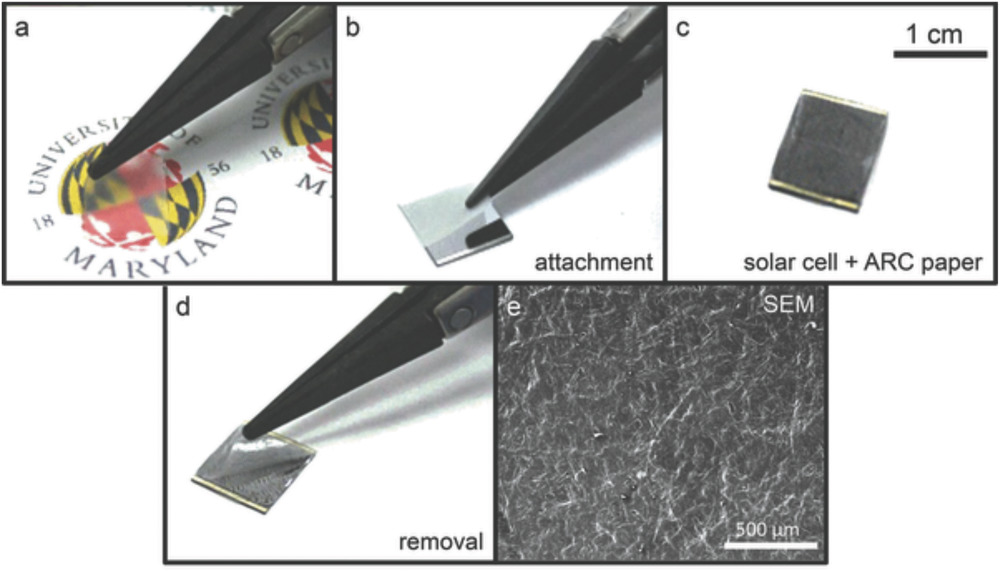
\includegraphics[width=0.75\linewidth]{fig2.png}
        \caption{a–c) Paper transfer and removal process. (a) The transparent cellulose paper used as an antireflection coating. (b) Transfer of the transparent paper antireflection coating on a GaAs solar cell. PVAc is used as a binding material. (c) The cell with the transparent cellulose paper antireflection coating on top. d) The paper can be removed as needed. e) A SEM image showing cellulose fibers within the transparent paper antireflection coating.\\
        \typeout{}
        [source: \url{https://doi.org/10.1002/aenm.201301804}]
        }
        % \label{fig:enter-label}
        
    \end{figure}

\end{frame}
\begin{frame}{Jak to naprawić za pomocą papieru II}
    \typeout{}

    \begin{figure}[h]
        \centering
                \begin{columns}
        \begin{column}{0.65\textwidth}
        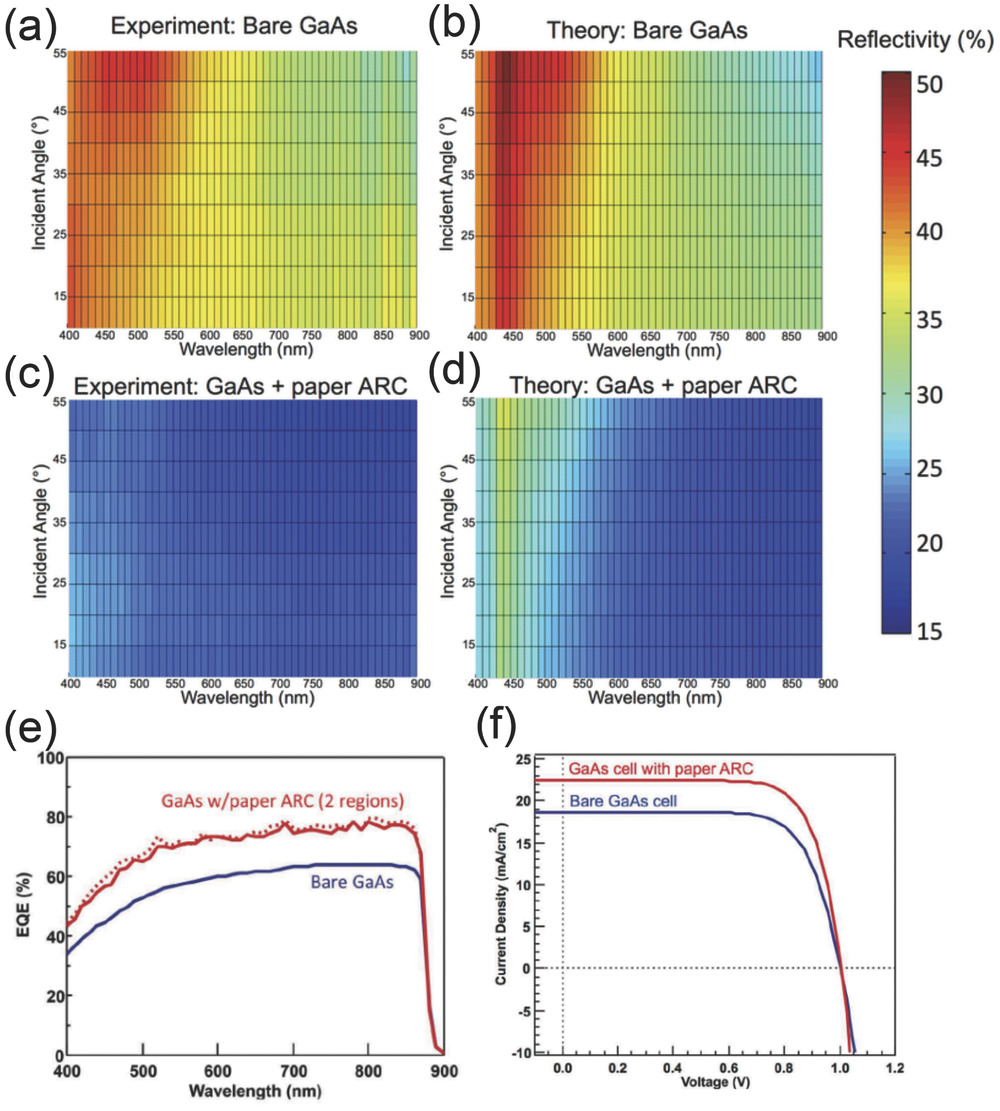
\includegraphics[width=\textwidth]{fig2f.jpg}
        \end{column}
        \begin{column}{0.35\textwidth}
         \caption{
         Transparent paper ARC reduces reflection over a wide range of incident angles and wavelengths. For the bare GaAs cell, contour plots of a) measured and b) calculated reflectivity as a function of incident angle \typeout{} and wavelength (from 400 nm to 900 nm) are in close agreement. The addition of a transparent paper ARC greatly reduces the measured reflection (c) over all angles and wavelengths. Calculations using an incoherent reflection model accurately predict the expected reduction of the reflectivity (d). Differences between the experiment and the calculations near $\lambda$ = 430 nm are predominately due to differences in the optical properties of the GaAs used and are independent of the paper ARC. 
        %  e,f) Measured electronic properties with and without the transparent paper-based antireflection coating on a GaAs solar cell. (e) EQEs are measured over the operational spectrum of a GaAs solar cell. Blue solid line indicates the measured EQE of a bare GaAs solar cell. Two different EQE measurements with the transparent paper-based ARC (red solid and dotted lines) confirm improved electronic characteristic induced by absorptivity enhancements. (f) Current–voltage characteristics with (red solid line) and without (blue solid line) the transparent paper-based ARC are determined. Increased light absorption within the active material improves the short-circuit current density by $\approx20\%$, which in turn results in $\approx24\%$ enhanced power conversion efficiency with a little enhancement in the fill factor.\\ 
         \typeout{}
	        [source: \url{https://doi.org/10.1002/aenm.201301804}]
         }
%         \label{fig:enter-label}
        \typeout{}
                        \end{column}
        \end{columns}
    \end{figure}
\end{frame}


\section{Obwody elektroniczne}

\begin{frame}{Obwody elektroniczne}

\begin{itemize}
\item problem: elastyczne układy elektroniczne
\item dodatkowe wymagania: przezroczystość, lekkość, ekologiczność
\item rozwiązanie: papier
\end{itemize}
    
\end{frame}

\begin{frame}{Jak to rozwiązać za pomocą papieru I }
    \begin{figure}
        \centering
        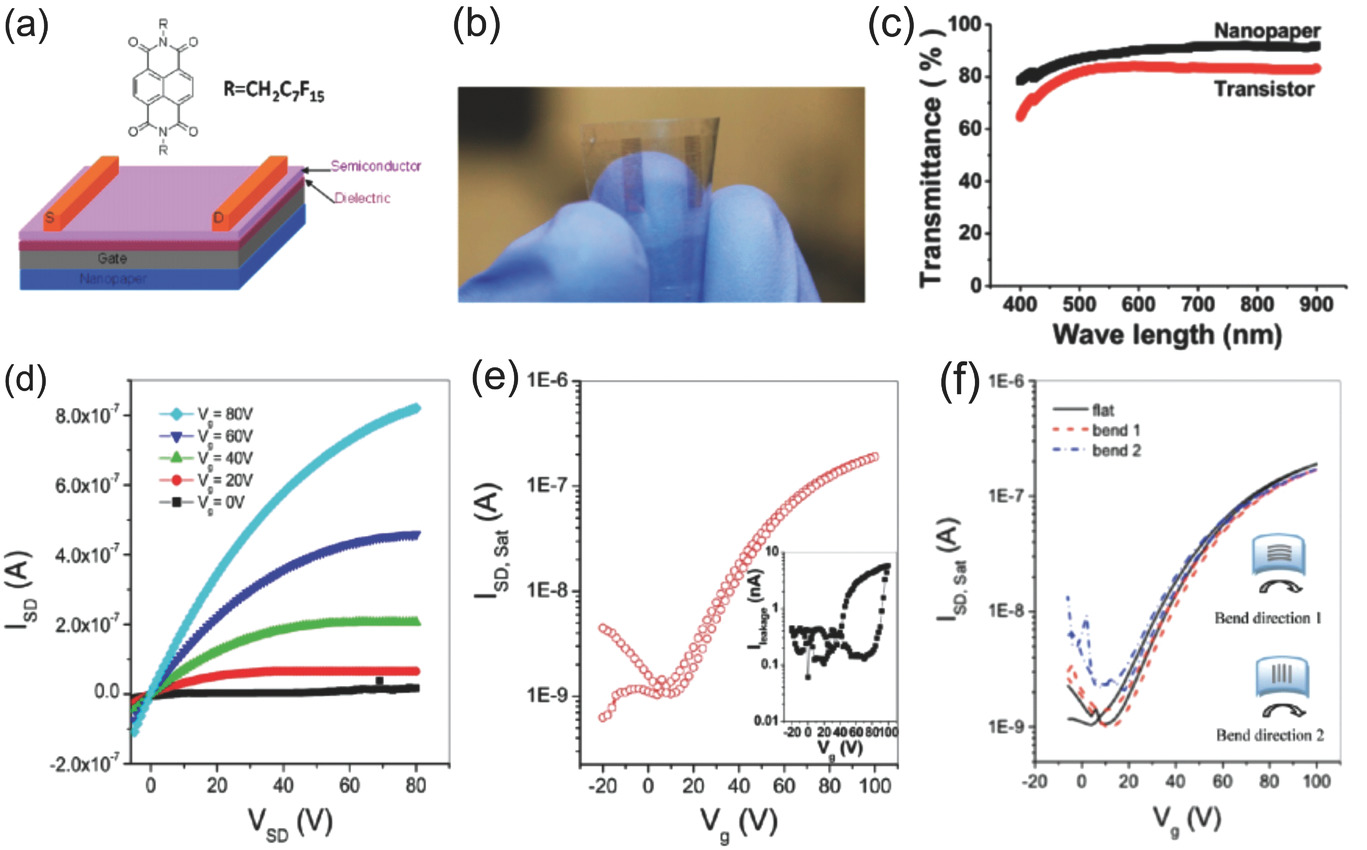
\includegraphics[width=0.7\textwidth]{fig4.jpg}
        \caption{a) Schematic showing the organic FET with a nanopaper substrate. Inset molecular structure shows F15-NTCDI semiconductor. b) A picture of the real fabricated device when it is bent. c) Measured optical transmittance of nanopaper used in this study and the fabricated device ($\approx$89\% and $\approx$84\% at a wavelength of 550 nm, respectively). d) Measured drain–source current–voltage characteristics ($I_{SD}$–$V_{SD}$) of the device for each applied gate voltage from 0 to 80 V. e) Transfer characteristic of the device when $V_{SD}$ = 10 V is measured. Inset shows how much gate leakage current is measured under gate voltage. f) Transfer characteristics of the device when it is bent. Black solid line, red dashed line, and blue dashed line represent measured transfer characteristics when the device is not bent, bent in vertical to the direction of conduction channel, and bent in parallel to the direction of conduction channel, respectively.\\ \typeout{}
        [source: \url{https://doi.org/10.1021/nn304407r}]}
        % \label{fig:my_label}
    \end{figure}
\end{frame}

\begin{frame}{Jak to rozwiązać za pomocą papieru II }
    \begin{figure}
        \centering
        \begin{columns}
        \begin{column}{0.5\textwidth}
        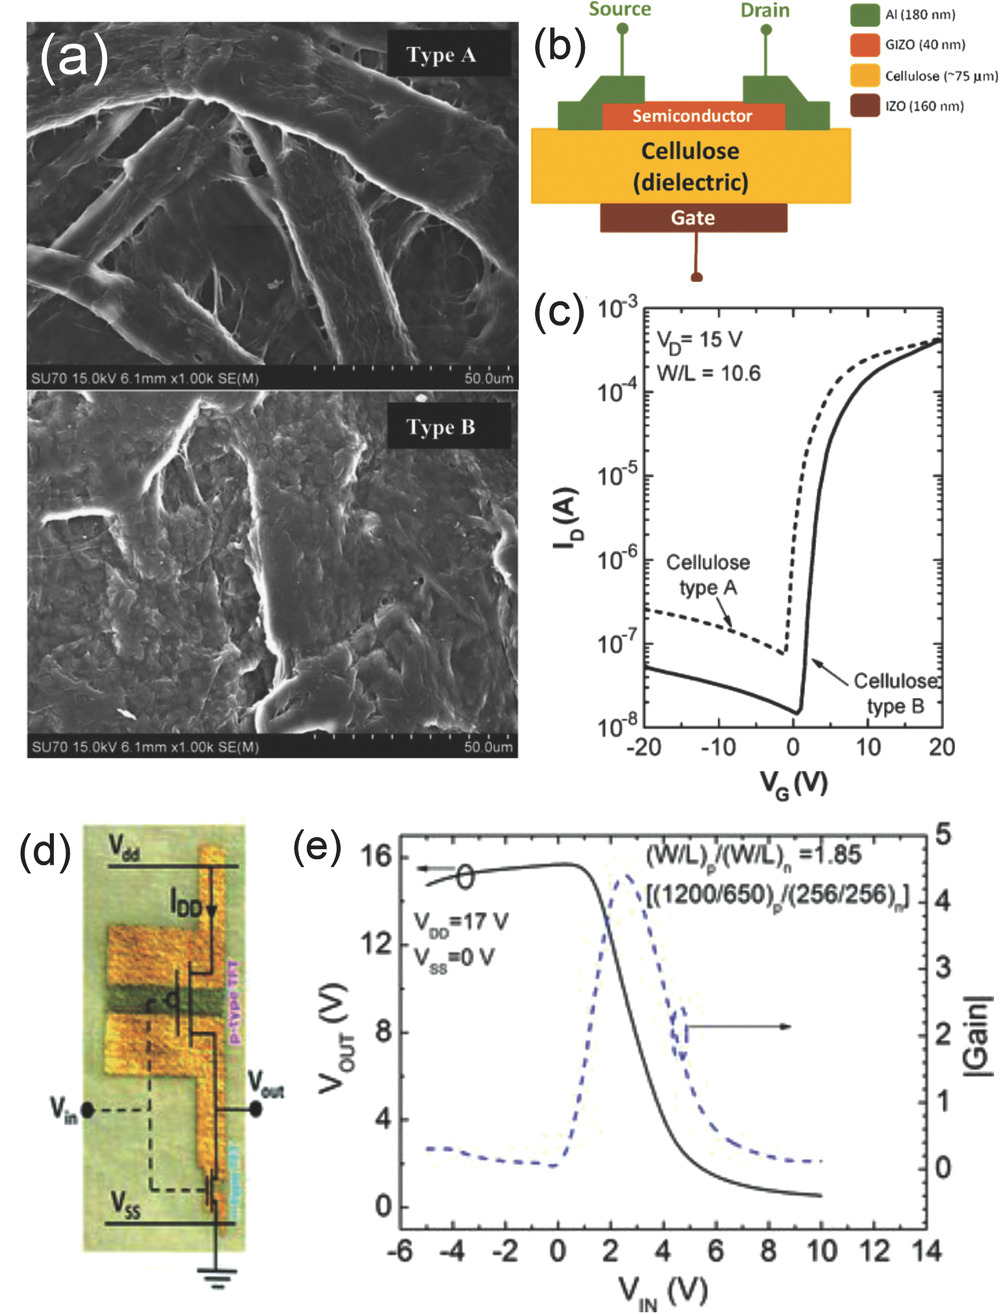
\includegraphics[width=\textwidth]{fig5.jpg}
        \end{column}
        \begin{column}{0.45\textwidth}
        \caption{a) SEM images showing two different types of papers. Type A has more porous cavities while type B is highly packed. b) Schematic of the field effect transistor using cellulose paper as a gate dielectric. c) I–V transfer characteristics measured at saturation region (drain voltage of 15 V) for devices with two different types of papers. Measurements are conducted at room temperature. d) An image showing paper-based CMOS inverter with p-type TFT (a gate width to length (W/L) ratio of 21.8) and n-type TFT (W/L ratio of 11.8). e) Device transfer characteristic of the paper-based CMOS inverter with the corresponding gain.\\ \typeout{}
        [source: \url{https://doi.org/10.1109/LED.2008.2001549}, \url{https://doi.org/10.1002/adfm.201202907}]}
        % \label{fig:my_label}
                \end{column}
        \end{columns}
    \end{figure}
\end{frame}

\section{Ekrany}

\begin{frame}{Ekrany}
    \begin{itemize}
\item problem: elastyczne ekrany
\item dodatkowe wymagania: przezroczystość, lekkość, ekologiczność
\item rozwiązanie: papier
\end{itemize}
\end{frame}

\begin{frame}{Ekranowanie}
    \begin{figure}
        \centering
        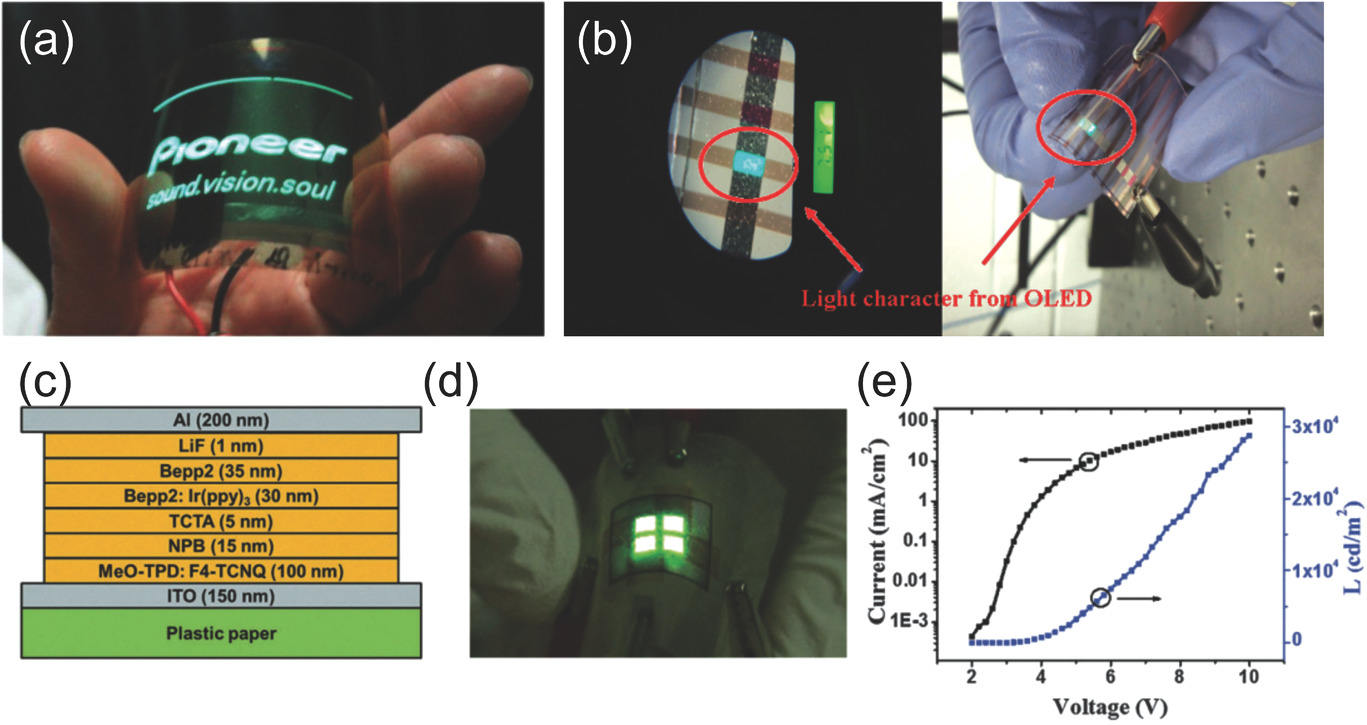
\includegraphics[width=0.8\textwidth]{fig8.jpg}
        \caption{a) A picture showing an operation of an OLED based on a flexible and transparent cellulose nanocomposite with low coefficient of thermal expansion. b) A picture showing an OLED on bacterial cellulose nanocomposite. The fabricated OLED can emit light even when it is bent. c–e) The OLED on plastic-paper hybrid substrate. (c) Schematic showing the layer information of the device. (d) The OLED atop plastic-paper hybrid substrate operates well when it is bent, confirming its shape stability and flexibility. (e) Current and light output efficiency are determined as a function of operation voltage.\\\typeout{}
        [sources: \url{https://doi.org/10.1016/j.compscitech.2009.04.017}, \url{https://doi.org/10.1016/j.indcrop.2011.06.025}, \url{https://doi.org/10.1039/C6EE01011C}]}
        % \label{fig:my_label}
    \end{figure}
\end{frame}

\section{Magazynowanie energii}

\begin{frame}{Magazynowanie energii}

\begin{itemize}
    \item problem: elastyczne, tanie, cienkie magazyny energii
\end{itemize}
    
\end{frame}

\begin{frame}{Papier}
        \begin{figure}
        \centering
        \begin{columns}
        \begin{column}{0.55\textwidth}
        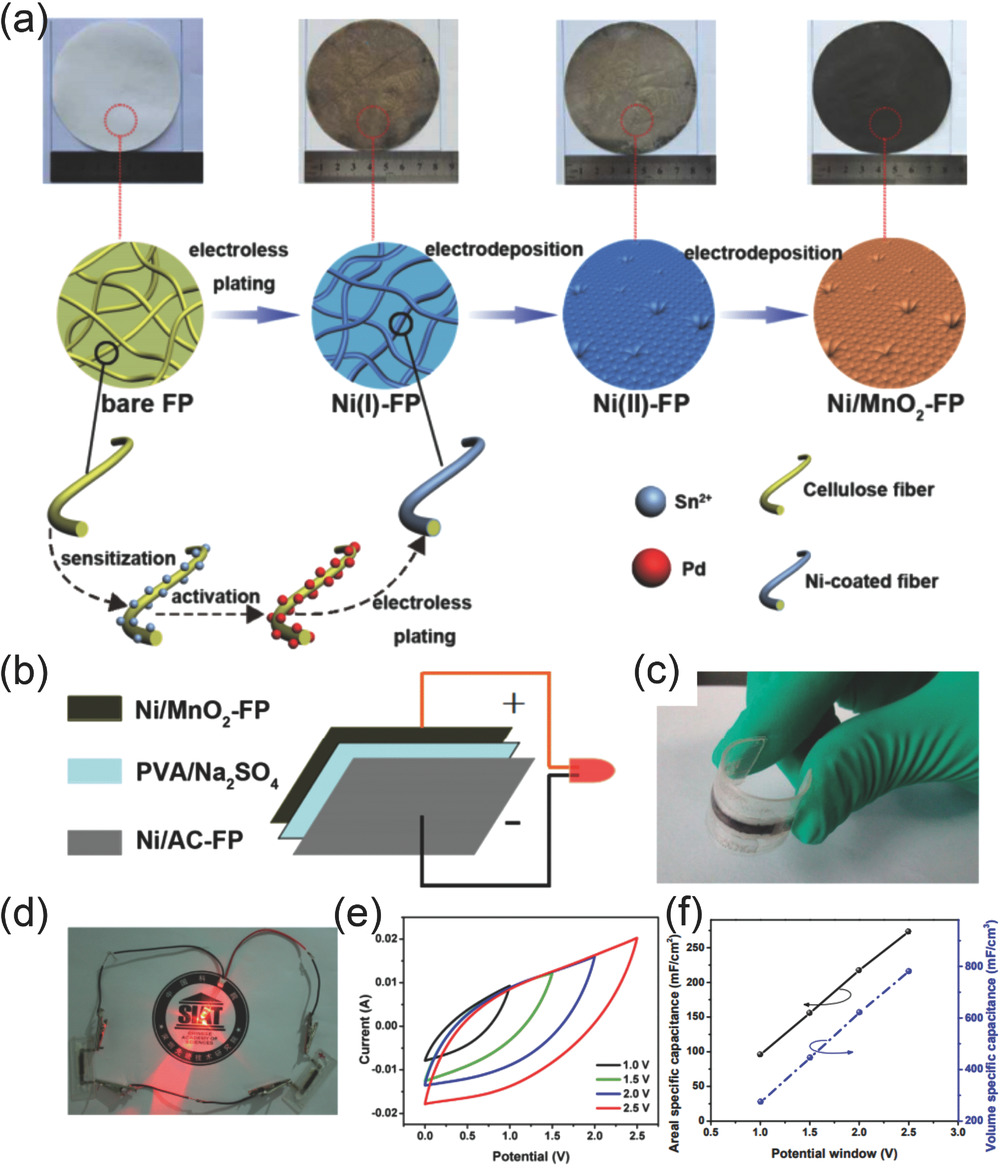
\includegraphics[width=\textwidth]{fig9.jpg}
        \end{column}
        \begin{column}{0.4\textwidth}
        \caption{a) Schematic showing the fabrication process of a flexible Ni/MnO2-FP positive electrode. b) Schematic showing the device constructed with an Ni/MnO2-FP positive and an Ni/AC-FP negative electrodes with PVA/Na2SO4 electrolyte. c) A picture shows the device's mechanical stability. d) A picture shows an LED powered up by two supercapacitors connected in series. e) Measured CV curves confirming the good electrochemical characteristic of the paper electrode-based supercapacitor. Measurements are performed at a scan rate of 100 \si{\milli\volt\per\second} when potential windows are varying from 1.0 to 2.5 V. f) Areal and volume capacitance are determined from the measured CV curves under different potential windows.\\ \typeout{}
        [source: \url{https://doi.org/10.1021/acsnano.5b06648}]}
        % \label{fig:my_label}
                \end{column}
        \end{columns}
    \end{figure}
\end{frame}

\section{Anteny}

\begin{frame}{Anteny}
    \begin{itemize}
        \item problem 1: anteny o dowolnych kształtach
        \item problem 2: anteny elastyczne
        \item dodatkowe wymagania: wytrzymałość, możliwość strojenia
    \end{itemize}
\end{frame}

\begin{frame}{Jak zrobić z papieru I}
        \begin{figure}
        \centering
        \begin{columns}
        \begin{column}{0.65\textwidth}
        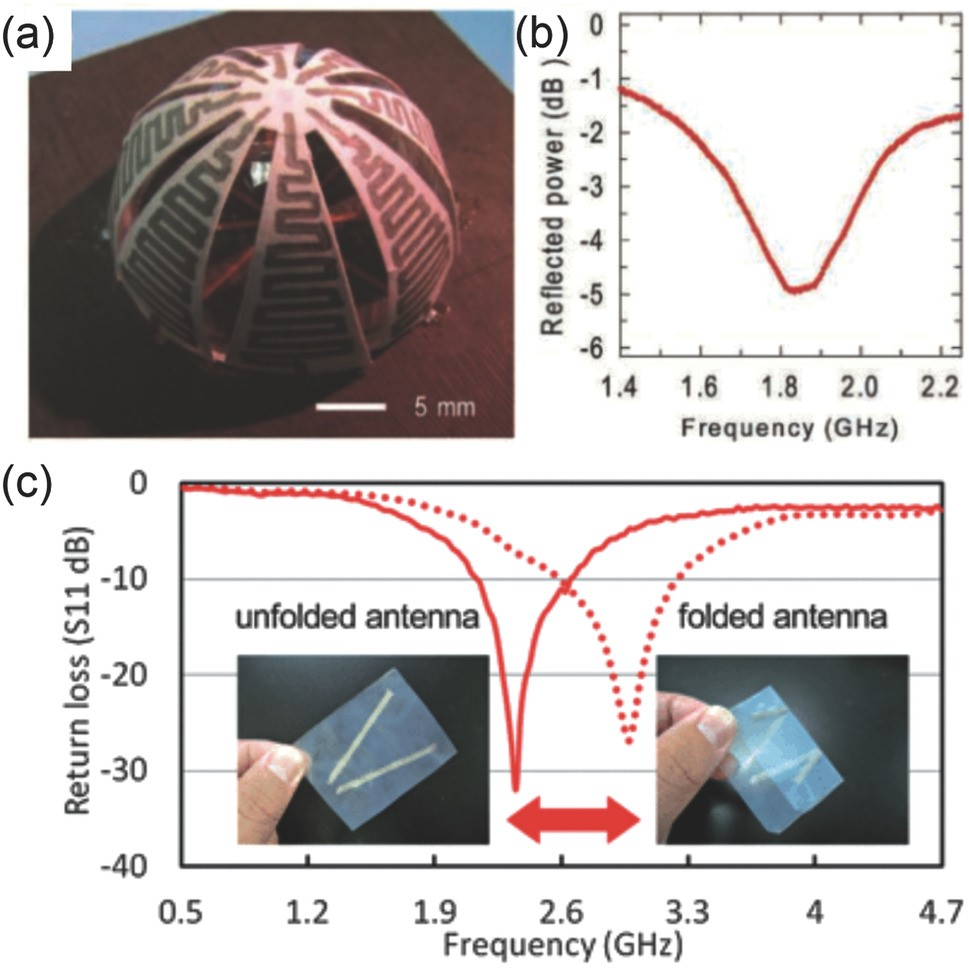
\includegraphics[width=\textwidth]{fig10a.jpg}
        \end{column}
        \begin{column}{0.3\textwidth}
        \caption{a,b) A 3D antenna based on paper substrate. (a) A picture showing the fabricated paper-based antenna patterned with a silver ink-contained ballpoint pen. (b) Measured reflected power confirms communication capability of the paper-based antenna. c) Return losses of paper-based foldable antennas can be tuned depending on how much the paper is folded. Solid line shows the return loss of an unfolded antenna and dotted line shows that of a folded antenna.   \typeout{}
        [sources: \url{https://doi.org/10.1002/adma.201101328}, \url{https://doi.org/10.1039/C3NR00231D}]}
        % \label{fig:my_label}
                \end{column}
        \end{columns}
    \end{figure}
\end{frame}

\begin{frame}{Jak zrobić z papieru II}
        \begin{figure}
        \centering
        % \begin{columns}
        % \begin{column}{0.6\textwidth}
        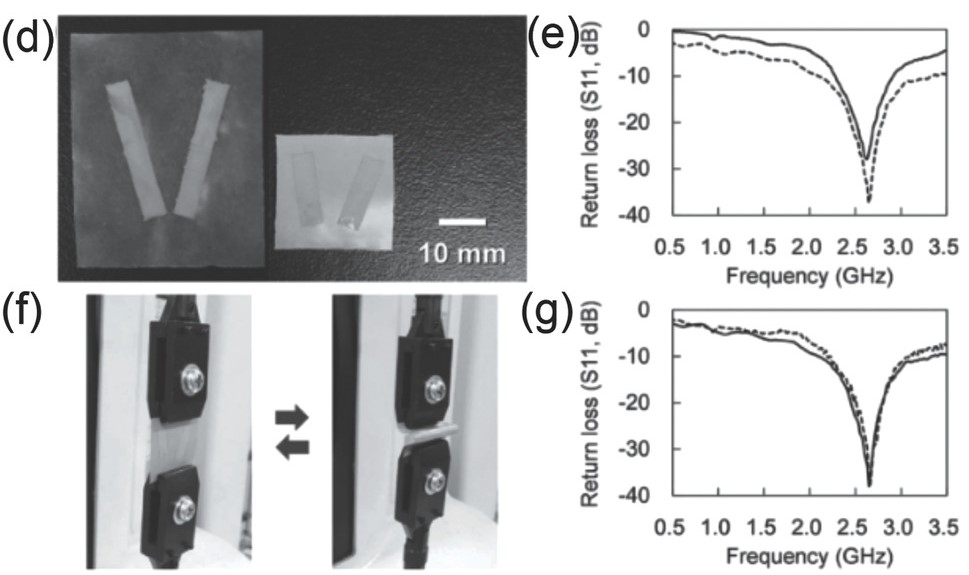
\includegraphics[width=0.8\textwidth]{fig10b.jpg}
        % \end{column}
        % \begin{column}{0.35\textwidth}
        \caption{d–g) A paper-based antenna for Wi-Fi communication. (d) Pictures showing a 30 mm long dipole antenna atop 50 µm thick nanopaper (left) and a 17 mm long dipole antenna atop 50 µm thick silver nanowire/nanopaper composite (right). (e) Return losses of the 30 mm long dipole antenna (solid line) and 17 mm long antenna on the silver nanowire/nanopaper composite (dashed line). (f) Pictures taken during bending of the nanopaper antenna and when it is restored. (g) The return loss of the nanopaper antenna before (solid line) and after (dashed line) 1001 cycles of bending test.\\  \typeout{}
        [source: \url{https://doi.org/10.1002/adma.201404555}]}
        % \label{fig:my_label}
                % \end{column}
        % \end{columns}
    \end{figure}
\end{frame}

\section{Podsumowanie}

\begin{frame}{Podsumowanie}
    \begin{itemize}
        \item papier znalazł wiele zastosowań w elektronice$^1$ ze względu na elastyczność
        \item jesteśmy w stanie zastosować przezroczysty papier 
        \item możemy wykorzystywać zarówno papier matowy (fotowoltaika) jak i błyszczący (ekrany)
        \item papier jest dobrym izolatorem, ale potrafimy zamienić go w przewodnik
        \item można wykorzystać elastyczność papieru do np. strojenia anten
    \end{itemize}
\end{frame}

\begin{frame}{Bibliografia}
\nocite{Ha_Fang_Zhitenev_2018}
                \printbibliography[heading=none]
\end{frame}

\begin{frame}{}

\begin{figure}

\centering
    \begin{tikzpicture}
      \duck[parrot, body=gray!30!yellow, head=gray!30!yellow, bill=red, tshirt=white!30!black, peakedcap=blue!50!black, ribbon=gray, bowtie=blue, crozier=brown!80!black]
      %\addwater{blue!50!cyan}
      \fill[cyan!20!white] (-1.4,1.8) ellipse (1.8 and 0.5);
  \fill[cyan!20!white] (-0.2,1.54) -- (0.2,1.35) -- (0.0,1.6) -- cycle;
	\node at (-1.4,1.8) {Dziękuję za uwagę};
    \end{tikzpicture}
    \end{figure}


    
    \begin{figure}
    \centering
    \qrcode[height=0.3\textwidth]{https://github.com/falcotinnunculus/przezrocza/tree/wladca/papier}\\
    {\tiny https://github.com/falcotinnunculus/przezrocza/tree/wladca/papier}

    \end{figure}
\end{frame}


% \appendix

% \begin{frame}{Współczynniki}
    
% \end{frame}

\end{document}